\begin{transitionframe}
\textbf{Part A:}

Informal Proof and Natural Deduction Proof
\end{transitionframe}


\begin{frame}{G\"odel's Manuscript (1970)}
ToDo: Improve Resolution
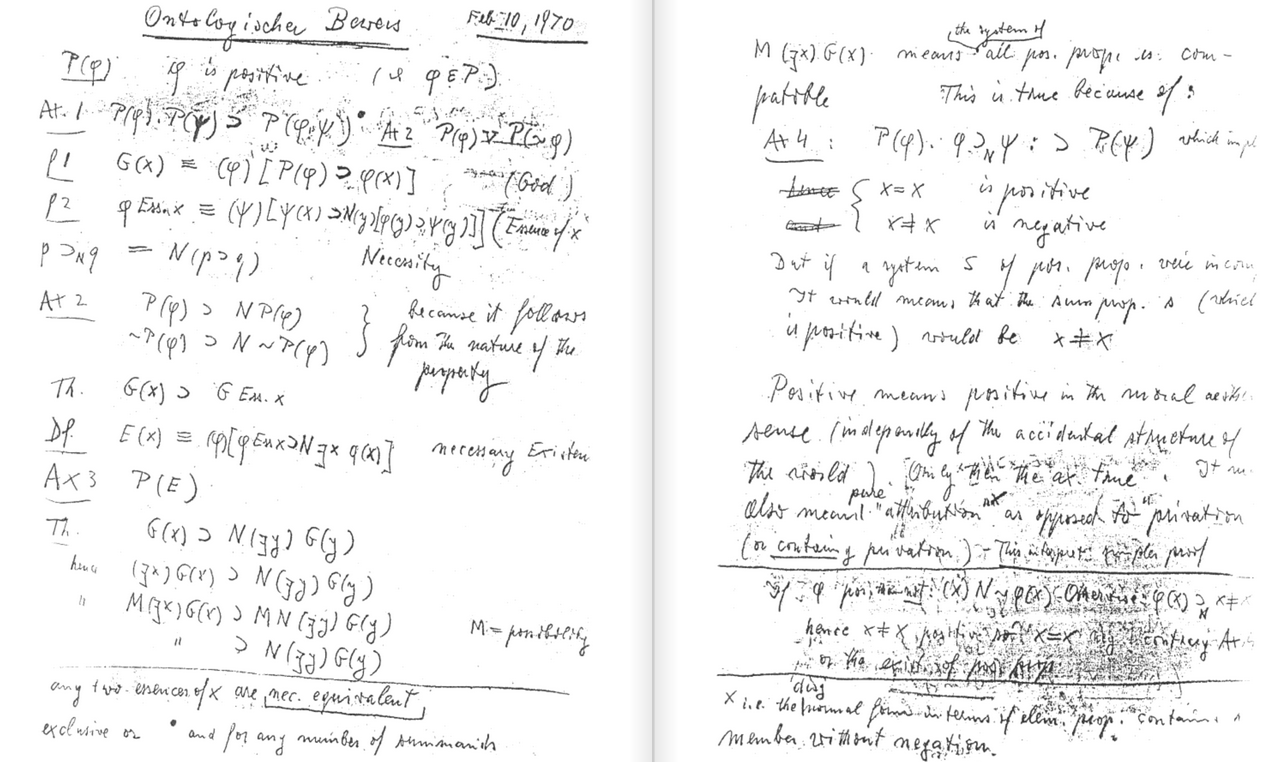
\includegraphics[scale=0.25]{Manuscript.png}
\end{frame}

\begin{frame}[shrink]{Versions}
    \begin{description}
		\item[A1] Either a property is positive or its negation is (never both):  \hfill 
		  $\all \phi [P(\neg \phi) \biimp \neg P(\phi)]$
		\item[A2] A property necessarily implied by a
		  positive property is positive: \phantom{b} \hfill 
		  $\all \phi \all \psi [(P(\phi) \wedge \nec \all x [\phi(x)
		  \imp \psi(x)]) \imp P(\psi)]$ 
		\item[T1] Positive properties are possibly exemplified: \hfill $\all \varphi [P(\varphi) \imp \pos \ex x \varphi(x)]$
		\item[D1] A \emph{God-like} being possesses all positive properties: \hfill
		  $G(x) \biimp \forall \phi [P(\phi) \to \phi(x)]$
		\item[A3]  The property of being God-like is positive: \hfill   $P(G)$
		\item[C\phantom{1}] Possibly, God exists: \hfill $\pos \ex x G(x)$
		\item[A4]  Positive properties are necessarily positive: \hfill 
		  $\all \phi [P(\phi) \to \Box \; P(\phi)]$
		\item[D2] An \emph{essence} of an individual is a property possessed by it and necessarily implying any of its properties:
		  \phantom{b} \hfill $\ess{\phi}{x} \biimp \phi(x) \wedge \all
		  \psi (\psi(x) \imp \nec \all y (\phi(y) \imp \psi(y)))$
		\item[T2]  Being God-like is an essence of any
		  God-like being: \hfill $\all x [G(x) \imp \ess{G}{x}]$ 
		\item[D3] \emph{Necessary existence} of an individual is \\ the necessary exemplification of all its essences: 
		  \phantom{b} \hfill $\NE(x) \biimp \all \phi [\ess{\phi}{x} \imp \nec \ex y \phi(y)]$
		\item[A5] Necessary existence is a positive property: \hfill $P(\NE)$
		\item[T3] Necessarily, God exists: \hfill $\nec \ex x G(x)$ 
		\end{description}

\end{frame}


\begin{frame}[shrink]{Proof Overview}

$$
\textbf{D1: } G(x) \equiv \forall \varphi. [P(\varphi) \to \varphi(x)]
$$

$$
\textbf{D2: } \ess{\varphi}{x} \equiv \varphi(x) \wedge \all \psi. (\psi(x) \imp \nec \all x. (\varphi(x) \imp \psi(x)))
$$

$$
\textbf{D3: } E(x) \equiv \all \varphi.[\ess{\varphi}{x} \imp \nec \ex y.\varphi(y)]
$$

\begin{prooftree}
\AXC{$\textbf{A3}$} \dashedLine
\UIC{$P(G)$}
		\AXC{$\textbf{A2}$} \dashedLine
		\UIC{$\all \varphi. \all \psi.[(P(\varphi) \wedge \nec \all x.[\varphi(x) \imp \psi(x)]) \imp P(\psi)]$}
					\AXC{$\textbf{A1a}$} \dashedLine
					\UIC{$\all \varphi. [P(\neg \varphi) \imp \neg P(\varphi)]$} \doubleLine
				\BIC{$\textbf{T1: } \all \varphi. [P(\varphi) \imp \pos \ex x.\varphi(x)]$} \doubleLine
	\BIC{$\textbf{C1: } \pos \ex x. G(x)$}
\end{prooftree}



\begin{prooftree}
						\AXC{$\textbf{A1b}$} \dashedLine
						\UIC{$\all \varphi. [\neg P(\varphi) \imp P(\neg \varphi)]$}
								\AXC{$\textbf{A4}$} \dashedLine
								\UIC{$ \all \varphi.[P(\varphi) \to \Box \; P(\varphi)] $} \doubleLine
							\BIC{$\textbf{T2: } \all y.[G(y) \imp \ess{G}{y}]$}
									\AXC{$\textbf{A5}$} \dashedLine
									\UIC{$ P(E) $} \doubleLine
								\BIC{$\textbf{L1: } \ex z. G(z) \imp \nec \ex x. G(x)$} \doubleLine
								\UIC{$\pos \ex z. G(z) \imp \pos \nec \ex x. G(x)$}
										\AXC{$\textbf{S5}$} \dashedLine
 										\UIC{$ \all \xi.[\pos \nec \xi \imp \nec \xi]$} \doubleLine	
									\BIC{$\textbf{L2: } \pos \ex z. G(z) \imp \nec \ex x. G(x)$}
\end{prooftree}

\begin{prooftree}
\AXC{$\textbf{C1: } \pos \ex x. G(x)$}
		\AXC{$\textbf{L2: } \pos \ex z. G(z) \imp \nec \ex x. G(x)$} \doubleLine
	\BIC{$\textbf{T3: } \nec \ex x. G(x) $}
\end{prooftree}

\end{frame}

\begin{frame}[shrink]{Natural Deduction Calculus}

\begin{unnamedCalculus}

\vspace{1em}

\s\s
\infer[\vee_E]{C}{A \vee B & \infer*{C}{\infer{A}{}} & \infer*{C}{\infer{B}{}}}
\s\s
\infer[\wedge_I]{A \wedge B}{A & B}
\s\s
\infer[\imp_I^n]{A \imp B}{ \infer*{B}{\infer[n]{A}{}} }

\vspace{2em}

\s\s
\infer[\vee_{I_1}]{A \vee B}{A}
\s\s
\infer[\wedge_{E_1}]{A}{A \wedge B}
\s\s
\infer[\imp_I]{A \imp B}{ B }

\vspace{2em}

\s\s
\infer[\vee_{I_2}]{A \vee B}{B}
\s\s
\infer[\wedge_{E_2}]{B}{A \wedge B}
\s\s
\infer[\imp_E]{B}{A & A \imp B}

\vspace{2em}

\s
\infer[\all_I]{\all x. A[x]}{ A[\alpha] }
\s
\infer[\all_E]{A[t]}{ \all x. A[x] }
\s\s
\infer[\ex_I]{\ex x. A[x]}{ A[t] }
\s
\infer[\ex_E]{A[\beta]}{ \ex x. A[x] }

\vspace{1em}

\s\s\s\s
$\neg A \equiv A \imp \bot$ 
\s\s\s 
\alert{\infer[\neg\neg_E]{A}{\neg\neg A}}

\vspace{1em}

\end{unnamedCalculus}

\end{frame}



\begin{frame}[shrink]{Natural Deduction Calculus}{Rules for Modalities}

\begin{unnamedCalculus}

\vspace{1em}

\s\s\s\s
\infer[\nec_I]{\nec A}{\alpha: \fbox{\infer*{A}{}} }
\s\s\s\s\s
\infer[\nec_E]{t: \fbox{ \infer*{}{A} }  }{\nec A}

\vspace{2em}

\s\s\s\s
\infer[\pos_I]{\pos A}{t: \fbox{\infer*{A}{}} }
\s\s\s\s\s
\infer[\pos_E]{\beta: \fbox{ \infer*{}{A} }  }{\pos A}

\vspace{2em}

\alert{$$\pos A \equiv \neg \nec \neg A$$}

\vspace{1em}

\end{unnamedCalculus}

\end{frame}



\begin{frame}{Natural Deduction Proofs}{T1 and C1}
\begin{prooftree}
        \AXC{\textbf{A2}} \dashedLine
        \UIC{$ \all \varphi. \all \psi.[(P(\varphi) \wedge \nec \all x.[\varphi(x) \imp \psi(x)]) \imp P(\psi)]$} \RightLabel{$\all_E$}
        \UIC{$ \all \psi.[(P(\rho) \wedge \nec \all x.[\rho(x) \imp \psi(x)]) \imp P(\psi)]$} \RightLabel{$\all_E$}
        \UIC{$(P(\rho) \wedge \nec \all x.[\rho(x) \imp \neg \rho(x)]) \imp P(\neg \rho)$} \doubleLine
        \UIC{$(P(\rho) \wedge \nec \all x.[\neg \rho(x)]) \imp P(\neg \rho)$}
                        \AXC{\textbf{A1a}} \dashedLine
                        \UIC{$\all \varphi.[ P(\neg \varphi) \imp \neg P(\varphi) ]$} \RightLabel{$\all_E$}
                        \UIC{$ P(\neg \rho) \imp \neg P(\rho) $} \doubleLine
                 \BIC{$ (P(\rho) \wedge \nec \all x.[\neg \rho(x)]) \imp \neg P(\rho) $} \doubleLine
                 \UIC{$ P(\rho) \imp \pos \ex x.\rho(x) $} \RightLabel{$\all_I$}
                 \UIC{$\all \varphi.[ P(\varphi) \imp \pos \ex x.\varphi(x) ] $}
\end{prooftree}

\begin{prooftree}
\AXC{\textbf{A3}} \dashedLine
\UIC{$P(G)$}
                 \AXC{\textbf{T1}} \dashedLine
                 \UIC{$\all \varphi.[ P(\varphi) \imp \pos \ex x.\varphi(x) ]$} \RightLabel{$\all_E $}
                 \UIC{$ P(G) \imp \pos \ex x.G(x) $} \RightLabel{$\imp_E$}
    \BIC{$\pos \ex x. G(x)$}
\end{prooftree}
\end{frame}



\begin{frame}{Natural Deduction Proofs}{T2 (Partial)}
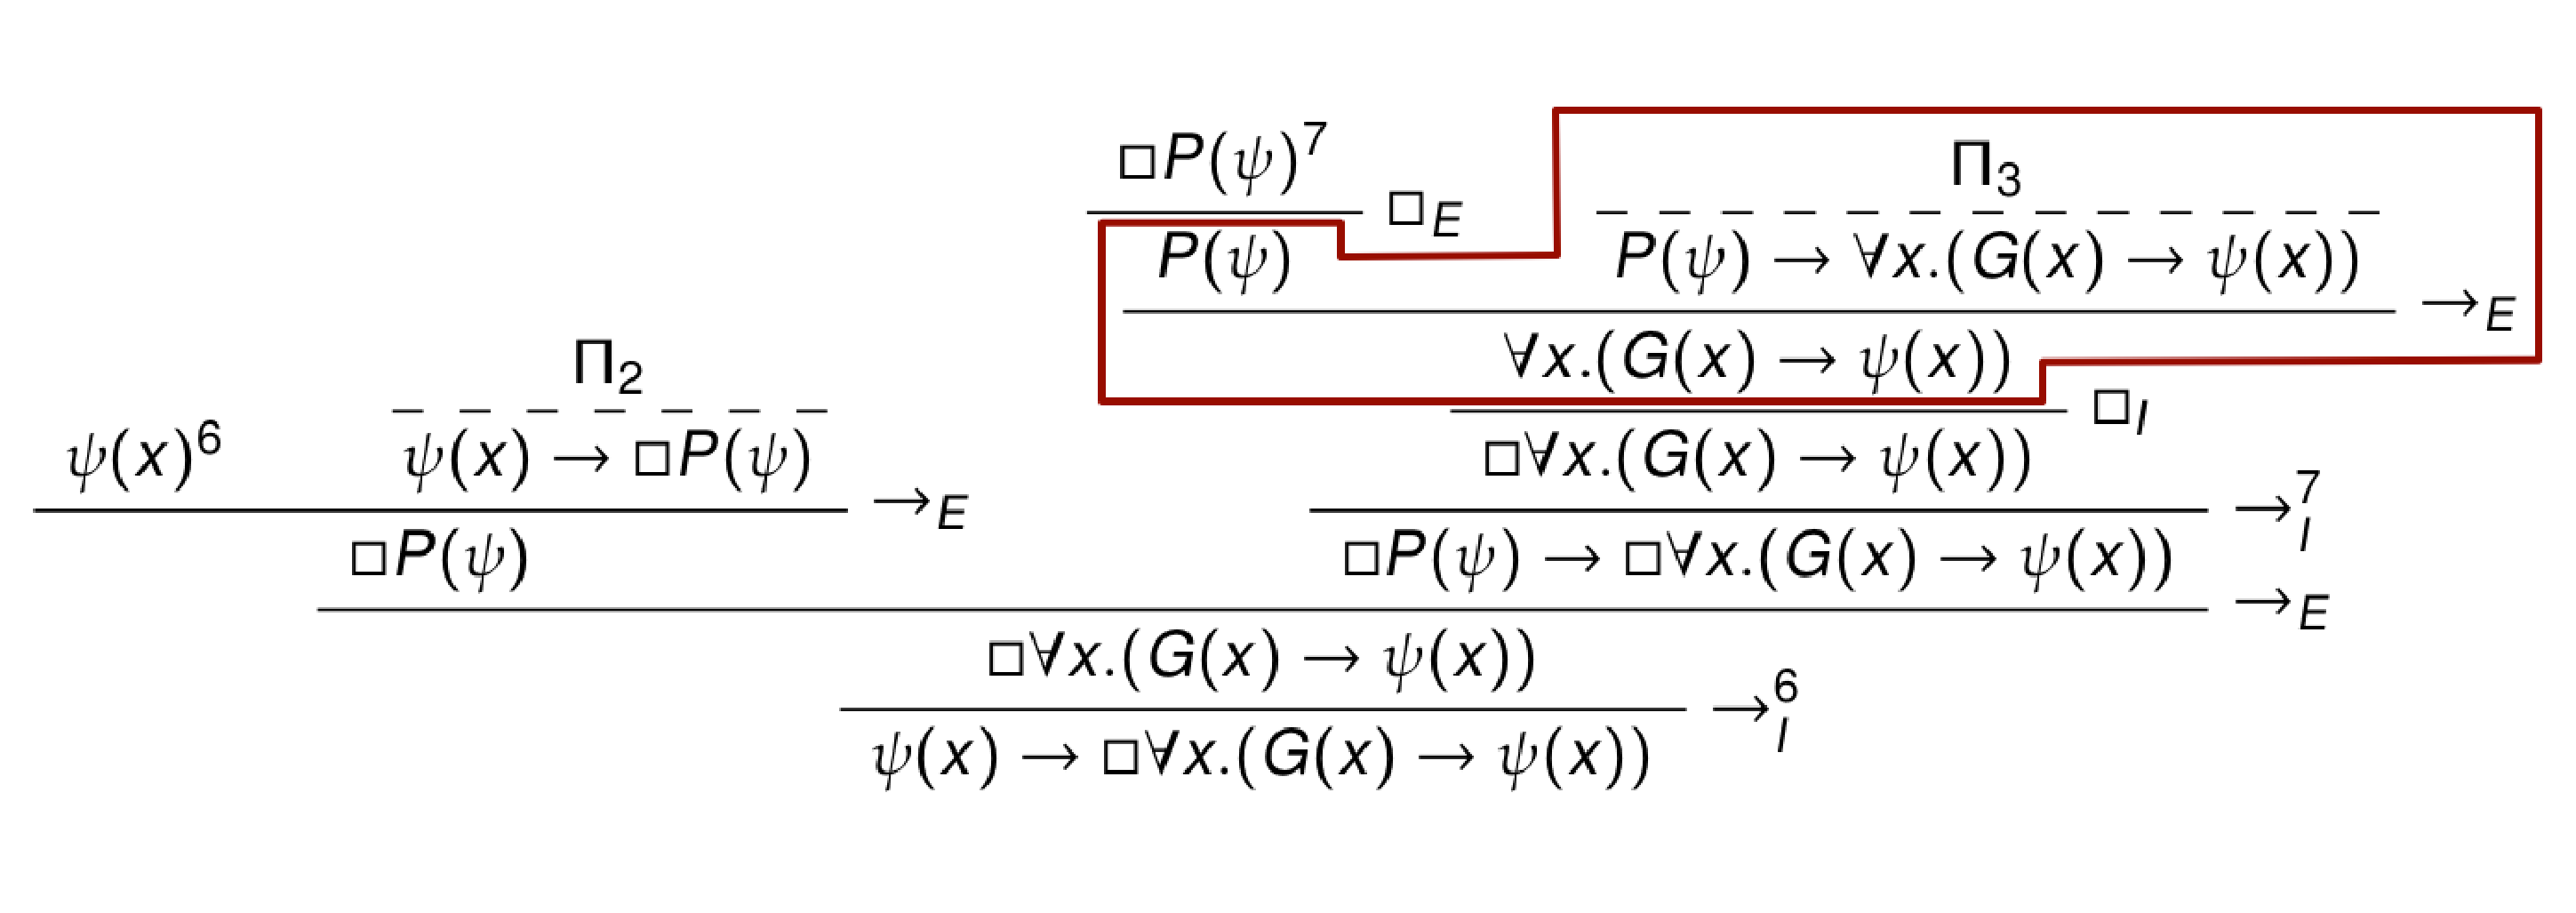
\includegraphics[scale=0.22]{ProofOfT2Boxed.pdf}
\end{frame}
